%----------------------------------------------------------------------------------------
%	CHAPTER 4: Ripa Blockchain
%----------------------------------------------------------------------------------------

\chapterimage{chapter_head_4_Dubai.jpg} % Chapter heading image
\chapter{The Ripa Blockchain}
\label{sec:theRipaBlockchain}
The RipaEx project will have its own blockchain called Ripa which will be run on the DPOS protocol and has the XPX 
token (\PHP symbol) running on it that will serve the five following purposes:
	\begin{enumerate}
		\item to list new cryptocurrencies on Ripa Exchanges
		\item to advertise new projects
		\item to buy RipaEx gadget on the RipaEx Store
		\item to pay for the sell of goods \& services on authorized resellers with our RipaEx POS (Point of Sale)
		\item to share liquidity between Ripa Exchanges in the same network
	\end{enumerate}

Ripa (XPX or \PHP) is a cryptocurrency derivate from ARK, Lisk, Crypti and BitShares with unique differences and improvements
for reaching the goal of shared liquidity between exchanges in the same Ripa network. This code however inherits the 
simplified interactions between ARK and other blockchain systems using DPoS as their consensus. This homogeneous codebase
allows for the potential to provide service bridges in the form of ARK-Lisk blockchain apps, along with any other additional 
systems provided by their blockchain administrators.

\vspace{5mm}
\textsc{\textbf{Ripa blockchain is an ARK fork and the use of a blockchain technology for the network of exchanges created will complete
the ripa ecosystem by permitting each exchange in the ripa network to share the same liquidity. We will always entrust ARK as our 
blockchain technology provider to merge their code into our latest features for what concerning the RIPA Blockchain}}

\vspace{5mm}

Explained the use of the Ripa Blockchain in the RipaEx ecosystem and explained the RIPA - ARK technological relations what is 
following are the specifications of the Ripa Blockchain derived/inherited from ARK.

\section{Delegated Proof of Stake Technology}
Ripa Blockchain, will inherits the Delegated Proof of Stake (DPoS) consensus system that was first introduced
by BitShares. This consensus algorithm was designed to eliminate the issues associated with Proof of Work (PoW), 
namely the centralization of computing power and the exponentially increasing waste of real world energy. While not
completely decentralized as it relies on consensus by a fixed number of elected delegates, it guarantees a better decentralization 
than Bitcoin. The consensus algorithm implementation is improved over time, evolving into an optimal consensus system.\\

The technical description of the Ripa blockchain is as follow:
\begin{enumerate}
	\item DPoS (Delegated Proof of Stake)
	\begin{itemize}
		\item 101 active forging Delegates
		\item Delegates selected by vote mechanism built into DPoS
		\item 115,000,000 XPX - Seeded Genesis Block
	\end{itemize}
	\item Multi-signature accounts
	\item Constant block reward
	\begin{itemize}
		\item 2 \PHP per block
		\item Inflation Rate (with 8s block times)
		\begin{itemize}
			\item 6.31\% for the first year
			\item 5.93\% the 2nd year
			\item 4.02\% the 10th year
		\end{itemize}
		\item 8-second block time
		\begin{itemize}
			\item Decreased block time possible with future upgrades to the core.
		\end{itemize}
		\item 25 transactions per block
		\begin{itemize}
			\item Increased via soft fork as needed.
		\end{itemize}
	\end{itemize}
	\item Routing tables
	\item SmartBridge data field for custom use and bridging blockchains (ARK Contract Execution Service)
	\item Batch transactions\footnote{Future upgrade: when ARK 2.0 will be released \label{note1}}
	\item Custom transaction fees\footnotemark[\value{footnote}]
	\item Native smart contract execution\footnote{Future upgrade: when ARK Virtual Machine will be released}
\end{enumerate}

\vspace{5mm}
\textsc{\textbf{As said Ripa blockchain is an ARK fork and we will entrust ARK as our blockchain technology provider to merge their 
code into our latest features for what concerning the RIPA Blockchain}}, features like:
\begin{itemize}
	\item \textbf{Scaling network} up to the level of major Credit Card networks with core upgrades
	\begin{itemize}
		\item Increasing the number of Forging Delegates
		\item Increasing the Block Size to include more transactions
		\item Implementation of pre-approval PBFT block concept testnet [codename:
		TwinChain]
		\item Routing tables, to minimize hops among nodes when blocks are broadcast
		\item Include forging with RIPA Uncles.	
	\end{itemize}
	\item \textbf{Two node types} is used to secure the RIPA network:
	\begin{itemize}
		\item \textbf{Relay nodes} - Nodes with full API functionality, acting as a back-end for the
		feature rich lite clients. Relay nodes do not collect any transaction fee and do
		not have the ability to Forge RIPA Blocks.
		\item \textbf{Forging nodes} - Nodes with reduced API functionality, decreasing the
		exposure to potential DDoS attacks on the RIPA Platform. Forging nodes are
		able to Forge RIPA and receive transaction fees.
	\end{itemize}
	\item \textbf{Official lite client} for network access is be provided shortly before the mainnet
	launch including desktop clients (Windows, MacOS, and Linux) and mobile clients
	(Android and iOS).
	\item \textbf{OffLine wallet creation}: the network itself does not use a Graphical User Interface by default. Any RIPA
	account can be created off-line and managed at no cost with a single device
	(computer, mobile phone, embedded ARM, IoT).
\end{itemize}

\section{Hierarchical Deterministic (HD) Wallets (BIP32)}
The structure of the public and private key generation follows the same specification
as Bitcoin. A custom implementation of BIP32 for Hierarchical Deterministic Wallets
is provided to RIPA users.

\section{Fees}
The fee for standard transactions is set at \PHP0.1 but the will be flexible in future releases of Ripa Blockchain.
At mainnet launch, a fee structure is provided out of the box to forging delegates with the following rules:
	\begin{itemize}
		\item Transaction \PHP0.1
		\item Vote \PHP1 (101 votes per transaction)
		\item Second Signature \PHP1
		\item Multi Signature \PHP1 per signature + \PHP1 per signing account
		\item Registering a delegate \PHP25.
	\end{itemize}
All fees are paid to the forging node which processes the block containing those fees.

\section{Ripa Delegates and Delegate Voting}
Any node running the core blockchain code wishing to become a forging node must
register their account within the RIPA network. The fee for this registration is set to
25 \PHP per delegate account registered.
RIPA incorporates a new DPoS voting system originally envisioned by the Crypti
Founders. The RIPA system fee is 1 \PHP per delegate vote. The voting weight of each
wallet will be split evenly between all delegates voted. For example:
\begin{itemize}
	\item If a wallet votes for one delegate, that delegate receives 100\% of the wallets
voting weight.
	\item If that wallet votes for an additional delegate, the entire vote weight is split
evenly between the two delegates at 50\%.
	\item By adding a third delegate, the voting weight splits again, and each of the
three delegates receives 33.333\% of the voting weight from that wallet.
\end{itemize}

The 101 forging nodes with the highest number of votes are eligible to Forge RIPA
blocks. This design eliminates the possibility that any single large RIPA holder or an
organization holding large percentages of RIPA are able to gain control over the
entire network by voting for all of their nodes into forging positions, thus effectively
taking complete control over that DPoS Blockchain. Votes from XPX Tokens held by
RIPA Crew may be used at RIPA Crew's discretion.

\section{Connecting Blockchains}
\subsection{ARK Bridged Blockchains (SmartBridge Technology)}
The ARK Platform does not provide direct support for sidechains or dapp databases.
Instead, a mechanism to bridge together blockchains is provided via a bridging
function built into ARK Core where any blockchain can send and receive trigger
function notices and informational data through the primary ARK network via
custom developed \textbf{SmartBridge(s)} and \textbf{Encoded Listeners}.
\begin{center}
	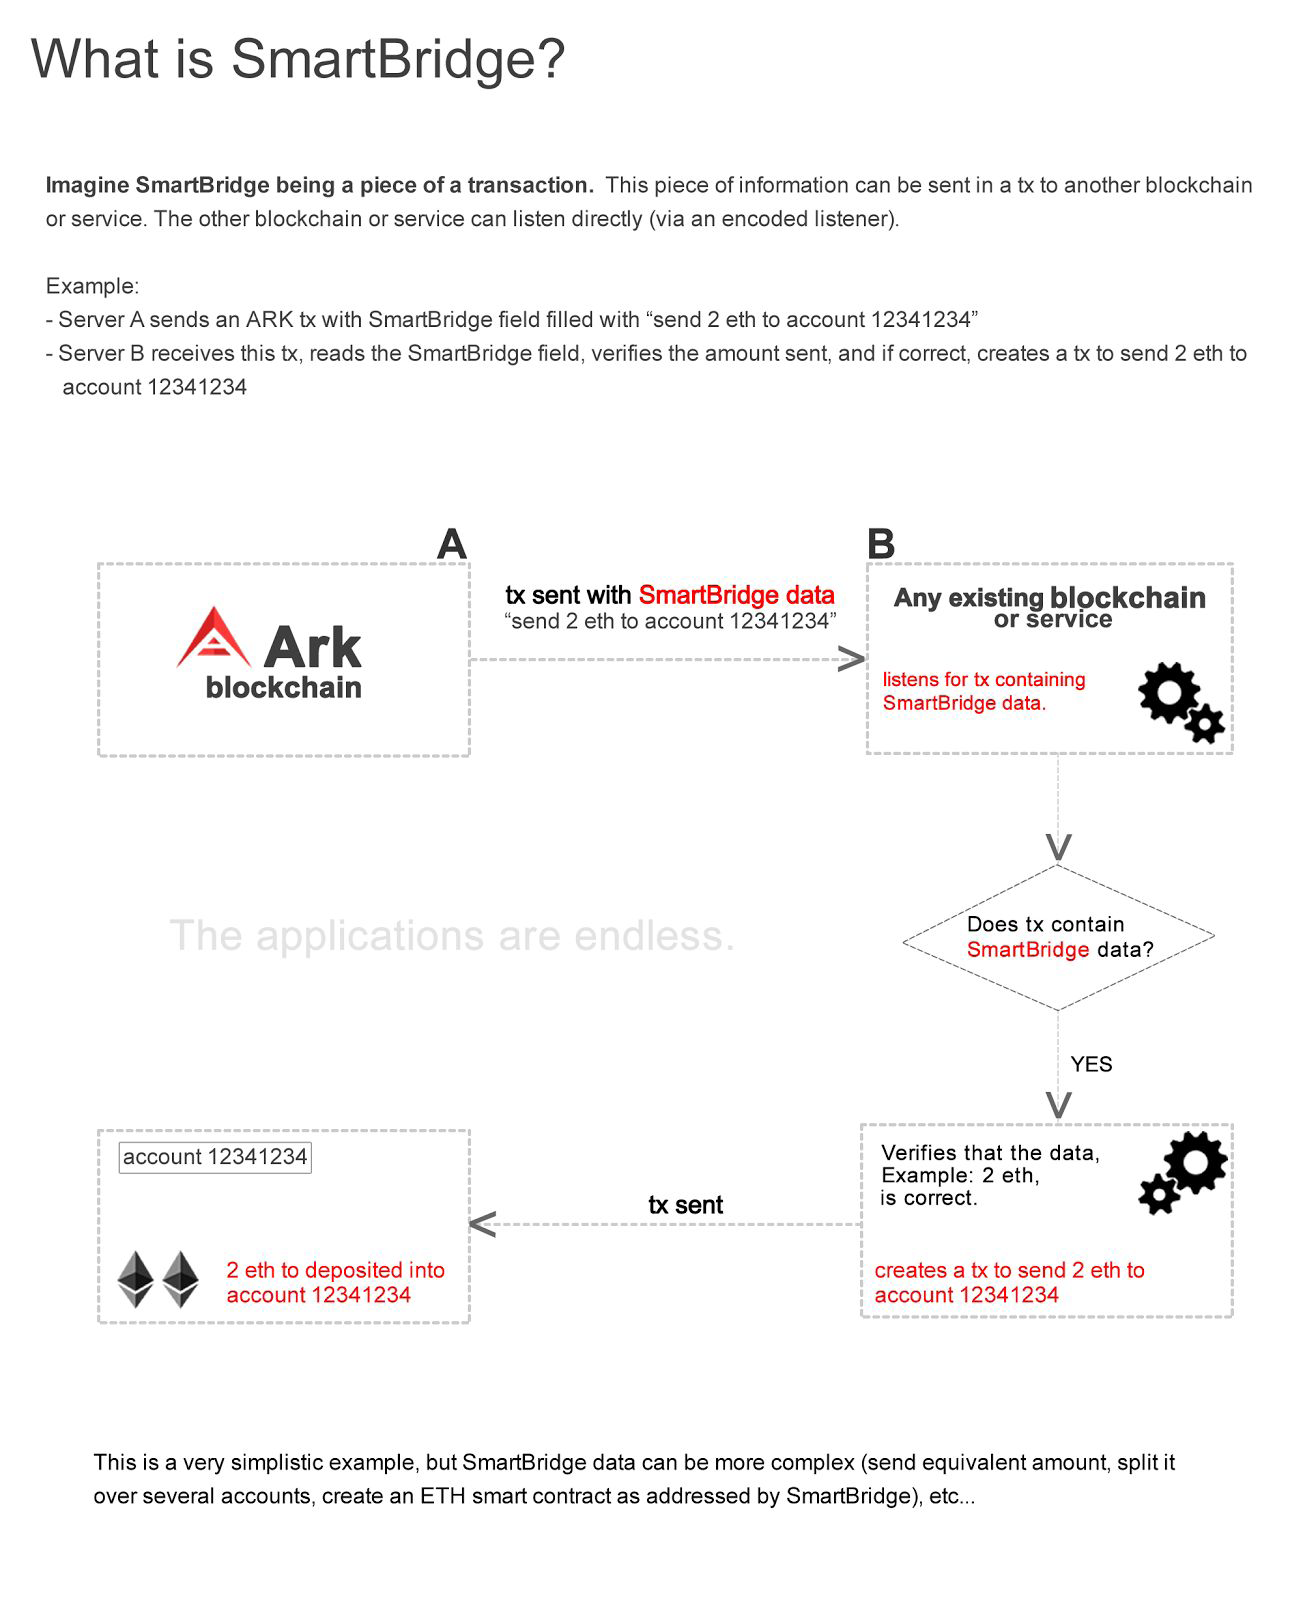
\includegraphics[width=\textwidth,height=\textheight,keepaspectratio]{ARKSmartBridge}
	\captionof{figure}{ARK SmartBridge Technology}
\end{center}

\subsection{A.C.E.S. - ARK Contract Execution Service}
ACES is a blockchain interoperability platform that provides simple protocols and tools for building a robust blockchain 
service marketplace.

ACES is composed mainly of the following three components:
\begin{itemize}
	\item \textbf{Listeners} ACES Listeners provide a way for all the different blockchain transaction events to be easily 
	consumed via a common REST-ful API. The API allows consumers to create subscriptions and receive blockchain events 
	in real-time using Webhook callbacks.
	\item \textbf{Services} ACES Services create and execute Service Contracts, which can be anything from uploading 
	a file to a storage blockchain, performing value transfers, creating smart contracts, executing code on 
	blockchain based computing platforms, or interacting with IoT hardware.
	\item \textbf{Marketplace Console} The ACES Marketplace Console is a consumer dashboard for searching and executing 
	service contracts listed on the Marketplace. ACES Service providers can list their service nodes using the Marketplace API.
\end{itemize}

\begin{center}
	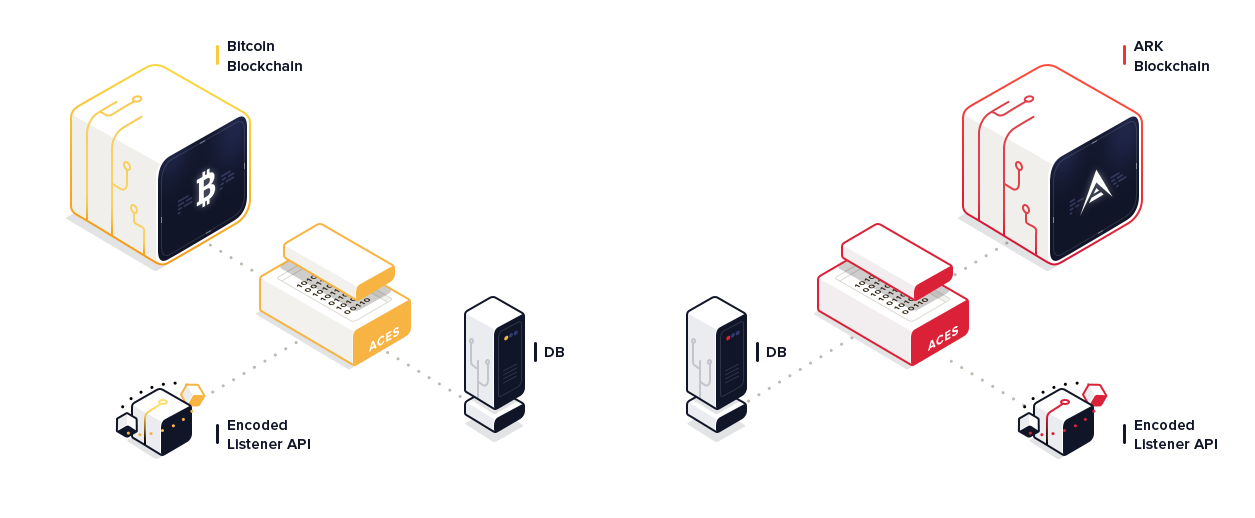
\includegraphics[width=\textwidth,height=\textheight,keepaspectratio]{ACES}
	\captionof{figure}{ARK-BTC A.C.E.S. SmartBridge Implementation Overview}
\end{center}

\section{Ripa Liquidity Service Provider (R.L.S.P)}
Using the SmartBridge technology RipaEx will build a mechanism to share liquidity between all the exchanges in the Ripa network
by writing the single exchange orderbook in the Ripa Blockchain and by executing order matching between all exchanges in the network.

In this way you can have the benefits of a decentralized orderbook (like liquidity) with the benefits of a centralized exchange (like
platinum customer support and FIAT exchange).

\section{Ripa Community Fund}
To permits the birth of new exchanges in the Ripa network a Ripa Community Fund - RCF - is created with the following characteristics:
\begin{itemize}
	\item \textbf{Starting Principal}: the RCF will have a starting operating capital of 5\% (5,750,000 \PHP) of the genesis block
	\item \textbf{Recurring Participation}: each delegate will contribute to the RCF with 5\% of its forged XPXs
\end{itemize}
\vspace{5mm}
To obtain funds from the RCF to start your own Ripa Exchange you will submit your proposal in the official RCF section in the Ripa forum at
anytime after the first Ripa Exchange instance will be operational.
